\documentclass[thesis.tex]{subfiles}

\title{Estimating duration in the presence of misclassification}
\author{Joshua Blake}
\date{\today}

\begin{document}

\ifSubfilesClassLoaded{
  \setcounter{chapter}{5}
}

\chapter{Survival analysis with false negatives} \label{imperf-test}

In \cref{E-perf-test}, a framework for analysing the CIS to produce estimates of the duration of detectability was developed.
However, the initial application of this framework produced an implausibly short estimate.
In this chapter, I identify this issue to be the result of false negatives, a form of misclassification bias, within the CIS (\cref{imperf-test:sec:problem}).
I then propose several models of false negatives (\cref{imperf-test:sec:simulate}) and extend the model of \cref{E-perf-test} to incorporate one of them (\cref{imperf-test:sec:modelling}).
After showing through simulation that the new model recovers the true duration distribution (\cref{imperf-test:sec:sim-study-results}), I apply it to the CIS data (\cref{imperf-test:sec:application}).
Finally, I discuss the results and further work in \cref{imperf-test:sec:discussion}.

The inclusion of false negatives into survival analysis is an area of much interest, especially in the application of tests for HIV in infants~\autocite[e.g.][]{brownBayesian,balasubramanianEstimation};
\textcite{piresIntervalMisclassify} provide a comprehensive review of approaches.
However, including false negatives with either doubly censored or truncated data has not been addressed.
The situation here requires both.



\section{The problem} \label{imperf-test:sec:problem}

Applying the method of \cref{E-perf-test} to CIS data estimates a median duration of less than 14 days, several days shorter than the estimates from \cref{E-ATACCC} (see \cref{imperf-test:fig:problem-cis-estimates}).
The \cref{E-ATACCC} estimates are more reliable over the first 2--3 weeks due to ATACCC's frequent data collection (see \cref{E-biology-data:sec:ataccc,E-ATACCC:sec:discussion}).
This suggests an issue in the estimation using CIS data.
\begin{figure}
  \makebox[\textwidth][c]{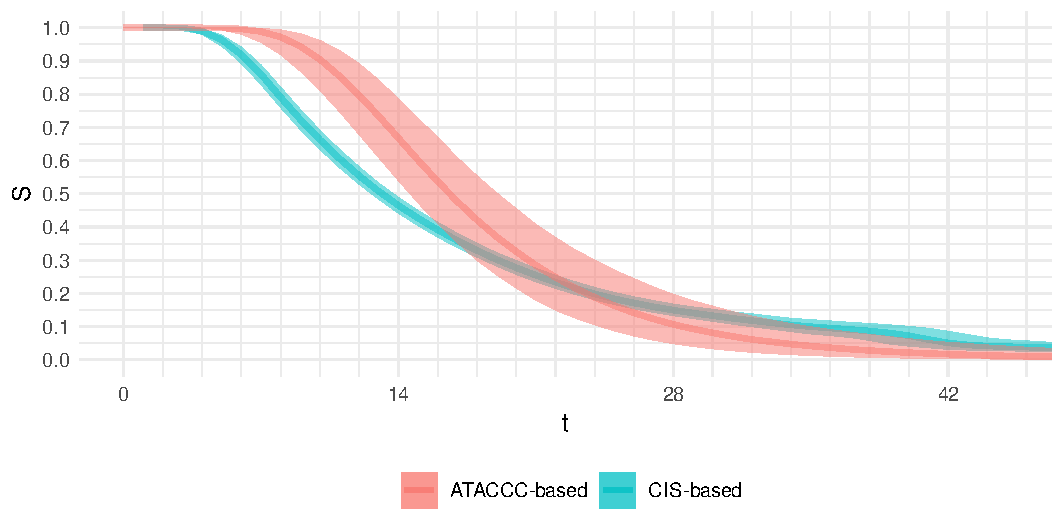
\includegraphics{cis-imperfect-testing/CIS_perfect}}
  \caption[Estimating survival using CIS data assuming perfect testing]{Estimates of the survival function using CIS data alongside the ATACCC-based estimates of \cref{E-perf-test}. \label{imperf-test:fig:problem-cis-estimates}}
\end{figure}

To investigate this further, I simulated \numprint{1000} datasets using the setup of \cref{E-perf-test:sec:simulation-study}.
The simulations produced far fewer single positive episodes than seen in the CIS data (compare the histogram with $\psens=1$ and the vertical line in \cref{imperf-test:fig:sim-single-pos}).
A single positive episode is an episode containing exactly one positive test; intuitively, these cause shorter estimates because the lower bound on the length of time the episode is one day, the shortest possible.
Specifically, if $j$ is a single positive episode then $O(j)$ allows $b_j = e_j = r_j^{(b)} = l_j^{(e)}$.
If this is true, then the duration is $d_j = e_j - b_j + 1 = 1$.
Additionally, short episodes are very likely to be undetected, which means that the design of the CIS cannot rule out many of them occurring.
% This produced the same pattern, that is estimating too many short episodes (not shown).

\Textcite{shenNonparametrica}, generalising \textcite{panNote}, studied the situation when only the terminating event is interval censored (\ie singly censored data) and left truncated.
They showed that the non-parametric maximum likelihood estimator is inconsistent if single positive episodes occur, and the survival function is severely biased downwards.

The CIS is a more complex setting, including double interval censoring and a complex pattern of undetected episodes (see \cref{E-perf-test:sec:problem}).
This means the result cannot simply be extended to the CIS, but still reinforces the intuition that single positive episodes are likely to be problematic.

% Discussion and interrogation of the data led me to
I hypothesised that the reason for the unexpectedly high number of single positive episodes (compared to simulation) was the presence of false negative results.
There are several strands of evidence supporting this hypothesis.
First, it is well known that RT-PCR testing can return false negatives  (see \cref{E-biology-data:sec:PCR}); I explicitly include them in the viral load model of \cref{E-ATACCC}.
Intermittent negatives (described in  \cref{E-biology-data:sec:PCR}) show that they occur within the CIS.
Furthermore, in \cref{imperf-test:sec:simulate}, I expanded the simulation study of \cref{E-perf-test:sec:simulation-study} to include false negatives.
This reproduced the CIS data more faithfully (see \cref{imperf-test:fig:sim-single-pos}) and exhibited the same issues when estimating the duration distribution (not shown).
\begin{figure}
  \makebox[\textwidth][c]{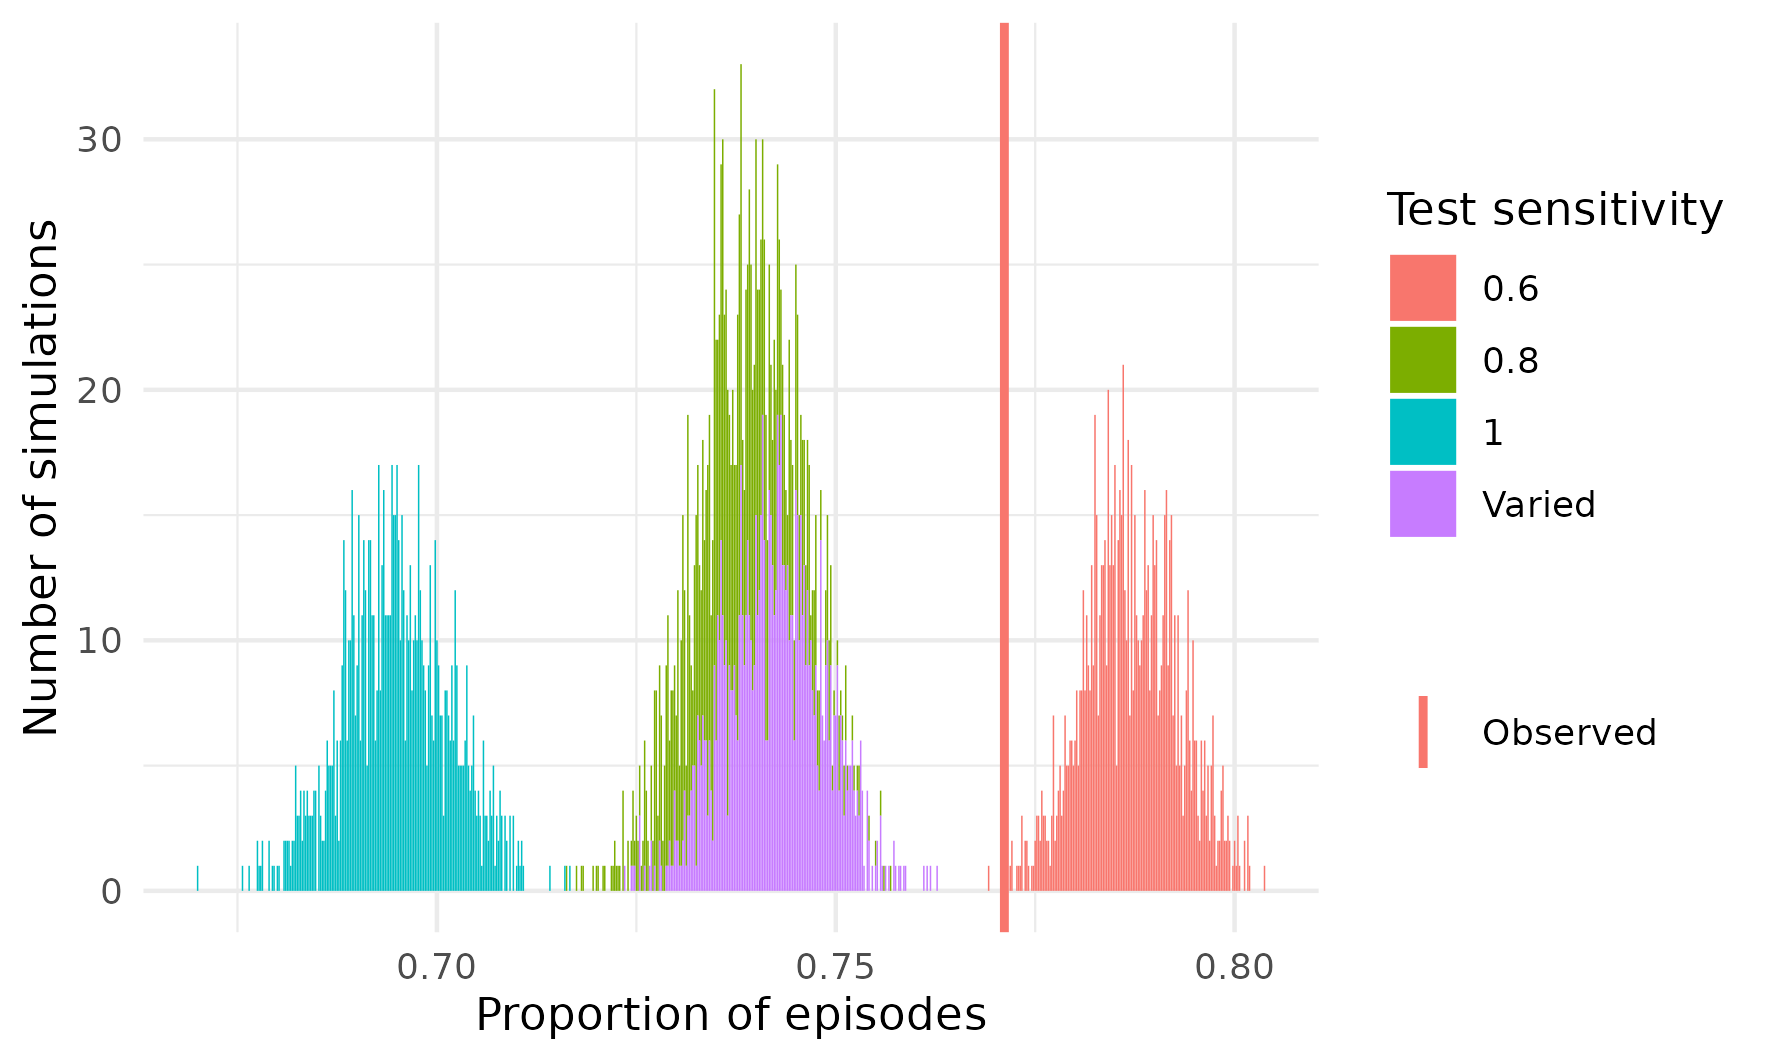
\includegraphics{cis-imperfect-testing/sim-single-positive-episodes}}
  \caption[Single positive episodes in CIS simulation]{%
    Proportion of detected episodes which have a single positive episode.
    y-axis is the number of simulations, out of \numprint{1000}, with the indicated proportion.
    Test sensitivity is $\psens$, with the varied test sensitivity referring to the model proposed in \cref{imperf-test:eq:variable-test-sensitivity}.
    The CIS data are shown as a vertical line.
  }
  \label{imperf-test:fig:sim-single-pos}
\end{figure}

\section{Generative model for false negatives} \label{imperf-test:sec:simulate}

In this section, I introduce a probabilistic model for the generation of false negatives.
Recall, from \cref{E-biology-data:sec:measurement-error}, that the test sensitivity, $\psens$, is the probability of a positive test result given that the individual is detectable.
The simplest model for false negatives is a constant $\psens < 1$.

Under this model, each test in a detectable individual generates an iid $\Ber(\psens)$ result where a one indicates a positive and zero indicates a negative.
As previously, tests in undetectable individuals are always negative.
I modified the simulation study from \cref{E-perf-test:sec:simulation-study} to generate test results in this way.

Following the modification, more single positive episodes are seen at lower values of $\psens$, with a value between 60\% and 80\% reproducing the number of single positive episodes observed in the CIS data (see \cref{imperf-test:fig:sim-single-pos}).
This is expected: a lower $\psens$ means that multiple positive tests are less likely, and hence the probability of a single positive episode is higher.

In \cref{E-ATACCC}, I estimated that $\psens$ is 95\% (95\% CrI: 93--96\%).
The daily testing this is based on means this is a reliable estimate during the period for which the individuals are followed-up.
The requirement for a much lower value of $\psens$ in the simulation study here suggests this model of false negatives is inadequate.

A better model would be to allow the rate of false negatives to vary over the course of an episode.
False negatives are more likely to occur when the viral load of an individual is low, because there is less virus in their body to sample.
In \cref{E-ATACCC}, this mechanism is incorporated by viewing negative tests as a left-truncation of the observation noise (see \cref{E-ATACCC:sec:observation-modification}).
This observation suggests that a model with a declining test sensitivity as a function of time since infection might be more suitable.

The CIS data provide evidence for the test sensitivity declining over the course of an episode.
\Cref{imperf-test:fig:bounding-cis-sensitivity} demonstrates this by using the following classification for test results.
\begin{enumerate}
    \item All positive results are true positives.
    \item All intermittent negatives are false negatives.
    \item The negative at the end of an episode is a possible false negative.
    \item All other negatives are true negatives.
\end{enumerate}
The classification assumes that the probability of two false negative tests at the end of an episode is negligible.
As test sensitivity is the proportion of individuals who should test positive that do so, it can be empirically calculated as number of true positives / (number of true positives + number of false negatives).
This can be bounded by assuming either all or none of the possible false negatives (group 3) are in fact false negatives.
I calculate the test sensitivity for each day, where the day of the first positive result in an episode is day zero.
Day zero is an unknown number of days after the episode's latent true beginning time.
% In \cref{imperf-test:fig:bounding-cis-sensitivity} we consider the values produced by assuming the negative following the last positive in an episode could be either a true or false negative as a function of time since the individual was detected (\ie the first positive test in the episode).
I generate broad bounds, suggestive of a declining test sensitivity over the course of an episode (see \cref{imperf-test:fig:bounding-cis-sensitivity}).
Small numbers of tests mean that the series is noisy near the start and the end, such as both bounds being 0 on some days after day 40.
However, the general trend is clear.
\begin{figure}
  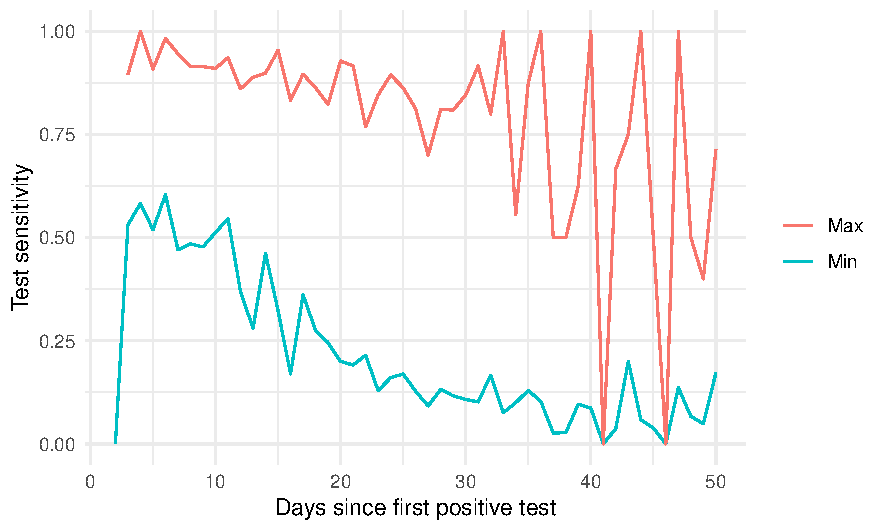
\includegraphics{cis-imperfect-testing/test-sens-bound}
  \caption[Bounding test sensitivity using CIS data]{
    Bounding the test sensitivity using CIS data as a function of time since the infection was detected.
  }
  \label{imperf-test:fig:bounding-cis-sensitivity}
\end{figure}

The following model allows simulating with a varying test sensitivity, allowing assessment of the inference procedure's sensitivity to this.
Through consideration of \cref{imperf-test:fig:bounding-cis-sensitivity}, and the interaction of false negatives due to viral load in \cref{E-ATACCC}'s results, I propose the following model.
\begin{equation}
  p_\text{sens}(t) = \begin{cases}
    0.9 - \frac{0.9-0.5}{50}t &t \leq 50 \\
    0.5 &t > 50
  \end{cases}
  \label{imperf-test:eq:variable-test-sensitivity}
\end{equation}
where $t$ is the number of days since infection.
The model consists of a linear decline in test sensitivity before a constant minimum point.

I simulate data under this model by, for each test in a detectable individual, calculating $\psens(t-b)$, where $t$ is the day of the test and $b$ is the day the episode began.
The result of the test is then a Bernoulli random variable, independent of all other considerations.
Incorporating this test sensitivity into the simulation gives much more similar results to the CIS data (see purple histogram in \cref{imperf-test:fig:sim-single-pos}).
Furthermore, it does not require low test sensitivities early in the infection, maintaining compatibility with the results in \cref{E-ATACCC}.

\section{Posterior density modification for false negatives} \label{imperf-test:sec:modelling}

In this section, I introduce a simple model of false negatives (\ie allowing $\psens < 1$) into the posterior density derived in \cref{E-perf-test:sec:model}; I continue to assume the probability of a false positive is negligible.
Using a simple model, in particular a constant test sensitivity, means calculating the likelihood remains tractable.
Additionally, I limit the number of permutations of false negative and true positive tests that I consider to have non-negligible probability.
Specifically, I assume that, if $i(j)$ is tested during infection episode $j$, either: the individual has a single false negative test and the episode ends before their next test, or the first test is a true positive test.
This assumption is reasonable because false negatives normally occur when the viral load is low, which is normally late in the infection episode.
For the same reason, I assume there is at most one false negative test following the final true positive test in the episode.

I start, in \cref{imperf-test:sec:notation}, by introducing some additional notation needed.
I then modify the components of the likelihood in \cref{imperf-test:sec:modifying-p_ia,imperf-test:sec:modifying-p_iu} to incorporate false negatives.

\subsection{Notation} \label{imperf-test:sec:notation}

Recall that, for an undetected infection episode, $O(j) = \emptyset$ and, for a detected episode, $O(j) = [l_j^{(b)}, r_j^{(b)}, l_j^{(e)}, r_j^{(e)}, i(j)]^T$ where $r_j^{(b)}$ is the day of the first positive due to infection episode $j$; $l_j^{(b)}$ is the day after the negative preceding this positive; $l_j^{(e)}$ is the day of the final positive due to infection episode $j$; $r_j^{(e)}$ is the day before the negative test following this positive; and $i(j)$ is the individual episode $j$ occurred in.
As $O(j)$ contains test results now subject to false negatives, it is now a random variable even after conditioning on $B_j$ and $E_j$ (previously it was deterministic).
Additionally, the results between the tests that bound episode $j$'s beginning and end times are also random and hence should enter into the likelihood.
For tractability, I consider only tests between the negative tests providing an upper bound on the length of episode $j$.

To do so, define a random vector $O'(j)$ with state space $\{\emptyset\} \cup \set{E}'$ which will replace $O(j)$ from \cref{E-perf-test}.
As before, $O'(j) = \emptyset$ if episode $j$ is undetected.
Otherwise, $O'(j) \in \set{E}'$ where $\set{E}' = \{ \vec{\nu}_1', \dots, \vec{\nu}_{N_E'}' \}$ augments the space $\set{E}$ with test results during the episode.
The elements of $\set{E}'$ are all $\vec{\nu}_k' = [\vec{\nu}_k, \vec{y}_k]^T$ where $\vec{\nu}_k \in \set{E}$ and $\vec{y}_k$ is a vector of test results for the relevant testing times, $\sched'_k = \{ t \in \sched_{i_k} \ssep r_k^{(b)} \leq t \leq r_k^{(e)} + 1 \}$.
To formalise the definition of $\vec{y}_k$, let $m_k$ denote the size of $\sched'_k$ and denote the elements of $\sched'_k$ by $t_{k,1} < \dots < t_{k,m_k}$.
Then, $\vec{y}_k \in \{0, 1\}^{m_k}$ and satisfies the following two conditions.
\begin{enumerate}
  \item The elements of $\vec{y}_k$ corresponding to the tests at times $r_k^{(b)}$ and $l_k^{(e)}$ are positive, \ie $y_{k,1} = y_{k,m_k-1} = 1$.
  \item The element of $\vec{y}_k$ corresponding to the test at time $r_k^{(e)} + 1$ is negative, \ie $y_{k,m_k} = 0$.
\end{enumerate}
These conditions are due to the construction of the intervals as positive and negative tests bounding the beginning and end times of the episode.

Let $p_k'$, $p_{ik}'$, $p_u'$, and $p_{iu}'$ have the same definition as $p_k$, $p_{ik}$, $p_u$, and $p_{iu}$ respectively except replacing $O$ with $O'$ and $\vec{\nu}_k$ with $\vec{\nu}_k'$, and conditioning on $\psens$.
As before, $p'_k = 1/\Ncis p'_{ik}$ and $p'_u = 1/\Ncis \sum_{i=1}^{\Ncis} p'_{iu}$.

\subsection{Deriving $p'_{ik}$} \label{imperf-test:sec:modifying-p_ia}

I will modify $p_{ik}$ to form $p_{ik}' = \prob(O'(j) = \vec{\nu}'_k \mid i(j) = i_k, \vec{\theta})$, taking into account false negatives.
I consider a mixture of two scenarios, whether the final test in $\sched'_{k}$ is a false negative, with the mixture probability determined by the test sensitivity.

Similar likelihoods have previously appeared in the literature~\autocite[e.g.][eq.\ (2)]{piresIntervalMisclassify}.
However, this prior work was for singly interval censored data; incorporating the double interval censored nature of the CIS data involves summing over the possible episode start times.

% I proceed by assuming that we have observed an arbitrary episode:
% \begin{align}
%   O'(j) = [[l_k^{(b)}, r_k^{(b)}, l_k^{(e)}, r_k^{(e)}, i(j)]^T, \vec{y}_k]^T.
% \end{align}
% I derive $p_k$ by considering the generating process that could have produced this episode.

By assumption, the negative test bounding the start of the episode, on day $l_k^{(b)}-1$, is a true negative.
True negatives occur with probability 1, and hence this test does not contribute to the likelihood.

As I assume that there are no false positives, the infection episode must span at least the period $[r^{(b)}_k, l^{(e)}_k]$, a period starting and ending with a positive test.
This includes all $t \in \sched'_k$ except $t = r_k^{(e)}+1$.
Therefore, the test results $\vec{y}_k$, except the test at $r_k^{(e)}+1$, are either true positives or false negatives.
This gives $t_+ = \sum_{l=1}^{m_k-1} y_{k,l}(t)$ true positives and $f_- = \sum_{l=1}^{m_k-1} (1 - y_{k,l}(t))$ false negatives.

Consider the negative test at $r_k^{(e)}+1$, the first negative after the start of the episode which may be a false negative.
It is a false negative if and only if the episode ends at or after the test, \ie $E_j > r_k^{(e)}$.
I proceed by considering whether this is the case and with $B_j = b$ known.

First, the case when $E_j \leq r_k^{(e)}$.
In this case, the test at $r_k^{(e)}+1$ is a true negative and the end of the episode is interval censored as in the previous chapter.
% In this case, the test at $r_k^{(e)} + 1$ is a true negative, as are all other tests not in $\sched'_{k}$.
The true negative occurs with probability 1, by the assumption of no false positives.
\begin{align}
&\prob(O'(j) = \vec{\nu}_k', E_j \leq r_k^{(e)} \mid B_j = b, i(j) = i_k, \psens, \vec{\theta}) \\
&= \prob(O'(j) = \vec{\nu}_k', l_k^{(e)} \leq E_j \leq r_k^{(e)} \mid B_j = b, i(j) = i_k, \psens, \vec{\theta}) &\text{the test at $l_k^{(e)}$ is positive} \\
&= \prob(O'(j) = \vec{\nu}_k' \mid l_k^{(e)} \leq E_j \leq r_k^{(e)}, B_j = b, i(j) = i_k, \psens, \vec{\theta}) \\
&\ \ \  \times \prob(l_k^{(e)} \leq E_j \leq r_k^{(e)} \mid B_j = b, i(j) = i_k, \psens, \vec{\theta}) \\
&= p_\text{sens}^{t_+} (1 - p_\text{sens})^{f_-} \left( S_{\vec{\theta}}(l_k^{(e)} - b + 1) - S_{\vec{\theta}}(r_k^{(e)} - b + 2) \right)
\label{imperf-test:eq:ll-ei-lt-ri}
\end{align}

Second, the case when $E_j > r_k^{(e)}$.
In this case, the test at $r_k^{(e)}$ is a false negative, occurring with probability $(1 - p_\text{sens})$.
To avoid having to consider tests after $r_k^{(e)}$, which could greatly complicate the likelihood, I model this case as the episode being right censored at $r_k^{(e)}$.
Taking the same approach as before:
\begin{align}
&\prob(O'(j) = \vec{\nu}_k', E_j > r_k^{(e)} \mid B_j = b, i(j) = i_k, \psens, \vec{\theta}) \\
&= \prob(O'(j) = \vec{\nu}_k' \mid E_j > r_k^{(e)}, B_j = b, i(j) = i_k, \psens, \vec{\theta}) \\
  &\ \ \  \times \prob(E_j > r_k^{(e)} \mid B_j = b, i(j) = i_k, \psens, \vec{\theta}) \\
&= p_\text{sens}^{t_+} (1 - p_\text{sens})^{f_-} (1 - p_\text{sens}) S_{\vec{\theta}}(r_k^{(e)} - b + 2)
\label{imperf-test:eq:ll-ei-gt-ri}
\end{align}

These expressions can now be used to derive $p'_{ik}$.
First, augment the data with $b$, and split into the cases just discussed, omitting the conditioning on $\psens$, $\vec{\theta}$, and $i(j) = i_k$:
\begin{align}
p_{ik}'
=& \prob(O'(j) = \vec{\nu}_k') \\
=& \sum_{b = l_k^{(b)}}^{r_k^{(b)}} \left( \prob(O'(j) = \vec{\nu}_k', E_j \leq r_k^{(e)} \mid B_j = b) + \prob(O'(j) = \vec{\nu}_k, E_j > r_k^{(e)} \mid B_j = b) \right) \prob(B_j = b). \\
\intertext{Now, substitute in \cref{imperf-test:eq:ll-ei-lt-ri,imperf-test:eq:ll-ei-gt-ri} and take out the common factor:}
=\ &  p_\text{sens}^{t_+} (1 - p_\text{sens})^{f_-} \\
 & \times \sum_{b = l_k^{(b)}}^{r_k^{(b)}} \left( S_{\vec{\theta}}(l_k^{(e)} - b + 1) - S_{\vec{\theta}}(r_k^{(e)} - b + 2) + (1 - p_\text{sens}) S_{\vec{\theta}}(r_k^{(e)} - b + 2) \right) \\ 
  & \times \prob(B_j = b \mid p_\text{sens}, \vec{\theta}) \\
=\ &  p_\text{sens}^{t_+} (1 - p_\text{sens})^{f_-} \\
  & \times \sum_{b = l_k^{(b)}}^{r_k^{(b)}} \left( S_{\vec{\theta}}(l_k^{(e)} - b + 1) - p_\text{sens} S_{\vec{\theta}}(r_k^{(e)} - b + 2) \right) \\
  & \times \prob(B_j = b \mid p_\text{sens}, \vec{\theta}).
\label{imperf-test:eq:pia-prime}
\end{align}
Note that if $p_\text{sens} = 1$ then $p_{ik}' = p_{ik}$ (see \cref{perf-test:eq:pia}).

If $\psens$ is fixed (\ie has a point prior) and $\prob(B_j = b \mid \psens, \vec{\theta}) \propto 1$ (as assumed in \cref{E-perf-test}) then:
\begin{align}
p_{ik}'
&\propto \sum_{b = l_k^{(b)}}^{r_k^{(b)}} S_{\vec{\theta}}(l_k^{(e)} - b + 1) - p_\text{sens} S_{\vec{\theta}}(r_k^{(e)} - b + 2).
\label{imperf-test:eq:pia-prime-constant}
\end{align}

\subsection{Deriving $p'_{iu}$} \label{imperf-test:sec:modifying-p_iu}

I now modify $p_{iu}$ to form $p_{iu}' = \prob(O'(j) = \emptyset \mid i(j) = i, \vec{\theta})$ to take into account false negatives.
Several mechanisms for episodes being undetected were considered when deriving $p_{iu}$ in \cref{E-perf-test:sec:prob-undetected}.
I now consider the additional mechanisms arising due to false negatives.
Specifically, episode $j$ could be undetected if the first test after $b_j$ is a false negative and then there are no subsequent positive tests.

This false negative would occur at the first test after the infection episode begins, on day $b_j + \tau_{\sched_{i(j)}}(b_j)$ (see \cref{E-perf-test:sec:prob-undetected}).
A false negative occurring requires that the episode has not yet ended but a negative still occurs.
The episode has not yet ended at the time of the test if $e_j = b_j + d_j - 1 \geq b_j + \tau_{\sched_{i(j)}}(b_j)$, that is the duration of the infection $d_j \geq \tau_{\sched_{i(j)}}(b_j) + 1$.
Conditional on the episode having not yet ended, the test result is negative with probability $1 - \psens$.

For there to be no subsequent positive tests, all tests up until day $e_j$ are false negatives.
By assumption, there is a negligible probability of two false negatives.
Therefore, this can only occur if the episode ends before another test.
Denote the number of days between $b_j$ and the test following the false negative as $\tau^2_{\sched_{i(j)}}(b_j) \stackrel{\text{def}}{=} \tau_{\sched_{i(j)}}(\tau_{\sched_{i(j)}}(b_j) + 1)$.
Then, the episode ends before this test if $d_j \leq \tau^2_{\sched_{i(j)}}(b_j)$.

Therefore, this mechanism causes episode $j$ to be undetected if all the following conditions hold.
\begin{enumerate}
    \item The episode would have been detected considering only the mechanisms in \cref{E-perf-test:sec:prob-undetected}. That is $\min(\sched_{i(j)}) < b_j \leq T_{i(j)}$ and $e_j \geq \tau_{\sched_{i(j)}}(b_j) + b_j$.
    \item The episode ends in the interval $[\tau_{\sched_{i(j)}}(b_j) + b_j, \tau^2_{\sched_{i(j)}}(b_j) + b_j - 1]$.
      Note that the lower bound here is exactly the bound on $e_j$ in the previous condition.
      Equivalently, $\tau_{\sched_{i(j)}}(b_j) + 1 \leq d_j \leq \tau^2_{\sched_{i(j)}}(b_j)$.
    \item A false negative occurs on day $\tau_{\sched_{i(j)}}(b_j) + b_j$. Conditional on the previous condition, this occurs with probability $1 - \psens$.
\end{enumerate}

The probability of this occurring, conditional on $B_j = b$ where $\min(\sched_{i(j)}) < b \leq T_{i(j)}$ is:
\begin{align}
&\prob \left(
    \tau_{\sched_{i(j)}}(b) + 1 \leq D_j \leq \tau^2_{\sched_{i(j)}}(b)
    \mid B_j = b, \vec{\theta} \right) (1 - \psens) \\
&= \left( S_{\vec{\theta}}(\tau_{\sched_{i(j)}}(b) + 1) - S_{\vec{\theta}}(\tau^2_{\sched_{i(j)}}(b) + 1) \right) (1 - \psens).
\end{align}
Summing over $b$, in the same way as \cref{perf-test:eq:piu}, gives:
\begin{align}
\zeta = (1 - p_\text{sens})\frac{1}{T} \sum_{b=\min(\sched_{i(j)}) + 1}^{T_{i(j)}} \left( S_{\vec{\theta}}(\tau_{\sched_{i(j)}}(b) + 1) - S_{\vec{\theta}}(\tau^2_{\sched_{i(j)}}(b) + 1) \right).
\label{imperf-test:eq:zeta}
\end{align}

$p_{iu}'$ is the probability of episode $i$ being undetected, considering both the mechanisms from \cref{E-perf-test} and the new mechanism here.
These mechanisms are mutually exclusive.
Hence, $p_{iu}'$ is the sum of these, $p_{iu}' = p_{iu} + \zeta$.
As in \cref{E-perf-test:sec:prob-undetected}, $1 - p_{iu}'$ is the required quantity.
\begin{align}
1 - p_{iu}'
=& 1 - p_{iu} - \zeta \\
=& \frac{1}{T} \sum_{b = \min \sched_{i} + 1}^{T_{i(j)}} S_{\vec{\theta}}(\tau_{\sched_{i}}(b) + 1) \\
&- (1 - p_\text{sens})\frac{1}{T} \sum_{b=\min(\sched_{i(j)}) + 1}^{T_{i(j)}} \left( S_{\vec{\theta}}(\tau_{\sched_{i(j)}}(b) + 1) - S_{\vec{\theta}}(\tau^2_{\sched_{i(j)}}(b) + 1) \right) \\
=& \frac{1}{T} \sum_{b=\min(\sched_{i(j)}) + 1}^{T_{i(j)}} \left( p_\text{sens} S_{\vec{\theta}}(\tau_{\sched_{i(j)}}(b) + 1) + (1 - p_\text{sens}) S_{\vec{\theta}}(\tau^2_{\sched_{i(j)}}(b) + 1)\right).
\label{imperf-test:eq:pit-prime}
\end{align}

\section{Simulation study} \label{imperf-test:sec:sim-study-results}

Here, I modify the simulation study in \cref{E-perf-test:sec:simulation-study} to assess several features of the statistical model I proposed in the previous section.
First, the ability to identify the survival function even with false negatives.
Second, the impact of misspecifying $\psens$, such as the assumption that it is constant.
Finally, the impact of the simplifying assumptions made in \cref{imperf-test:sec:modelling} for tractability.
These assumptions are that the negative at $l^{(b)}_j - 1$ is a true negative and that there is a negligible probability of missing an episode due to two false negatives.

Denote by $\psenss$ the test sensitivity value used when simulating the dataset, with $\psens = v$ indicating the varying test sensitivity, from \cref{imperf-test:eq:variable-test-sensitivity}, was used.
Denote by $\psensi$ the constant test sensitivity value assumed during inference.

I use one dataset from \cref{imperf-test:sec:simulate} for each $\psenss \in \{ 0.6, 0.8, 1.0, v \}$.
The simulation is otherwise unchanged from that in \cref{E-perf-test:sec:simulation-study}.
The number of single positive episodes in each of these conditions, compared to the number observed in the CIS data, is shown in \cref{imperf-test:fig:sim-single-pos}.

For each simulated dataset, I estimate the survival function using the posterior density proposed in \cref{imperf-test:sec:modelling} and assuming each $\psensi \in \{0.6, 0.8, 1.0\}$.
If $\psenss = \psensi$, I refer to $\psens$ as being correctly specified; otherwise, I refer to it as misspecified.
However, there is still some misspecification of the model to false negatives owing to the simplifying assumptions made.
The amount that the simplifying assumptions are violated increases as $\psenss$ decreases.

I use either the independent (vague) or model combination priors for the survival (described in \cref{E-perf-test:sec:parameters-priors}).
These were shown to be the best performing priors in \cref{E-perf-test:sec:results}.
Therefore, there are a total of 24 possible scenarios, although not all are shown.
These are each combination of: 4 simulated datasets, with the different values of $\psenss$; 3 values of $\psensi$; and 2 priors for the hazard.

When $\psens = 0.8$ and is correctly specified, the model recovers the true survival time well (see \cref{imperf-test:fig:constant-test-sensitivity}(B)).
The informative prior, in comparison to the vague prior, helps to overcome the misspecification due to the simplifying assumptions, moving the estimated survival function closer to its true survival time.
However, when $\psens = 0.6$, this is no longer the case (see \cref{imperf-test:fig:constant-test-sensitivity}(A)).
This is likely caused by too large a violation of the simplifying assumptions made in \cref{imperf-test:sec:modelling}.
\begin{figure}
  % \makebox[\textwidth][c]{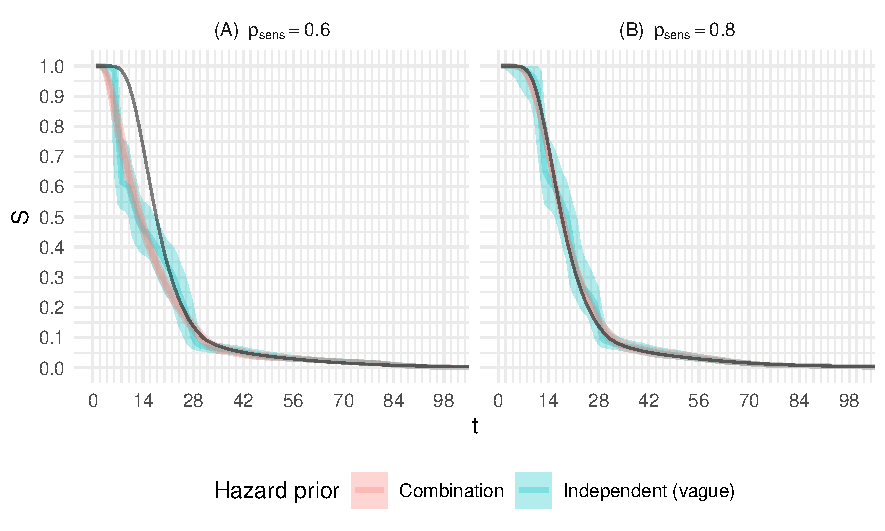
\includegraphics[width=1.2\textwidth]{cis-imperfect-testing/sim-constant-sensitivity}}
  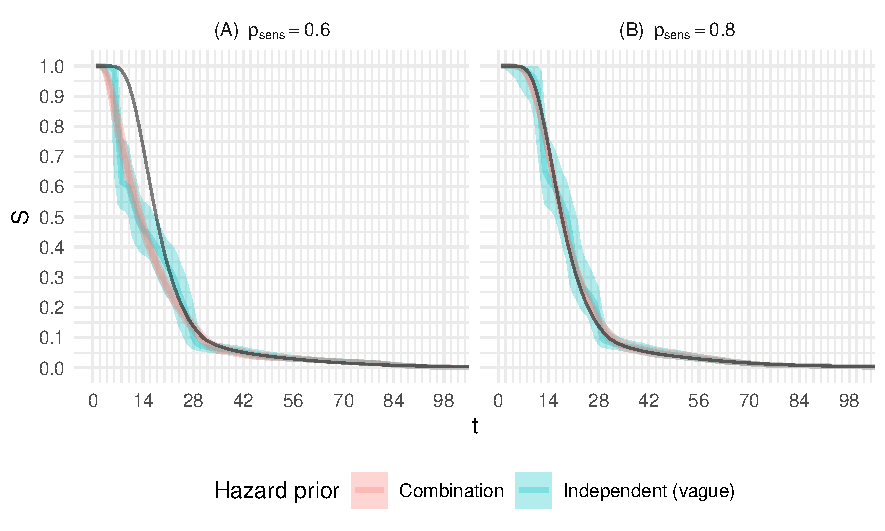
\includegraphics[width=\textwidth]{cis-imperfect-testing/sim-constant-sensitivity}
  \caption[Simulation study results with constant test sensitivity]{%
    Posterior (median and 95\% credible interval) of the survival time for the simulation study with $\psens$ correctly specified.
    The true survival time is shown in black.
  }
  \label{imperf-test:fig:constant-test-sensitivity}
\end{figure}

Next, I considered the consequence of $\psens$ being misspecified, I use the model combination prior because it is the better performing prior in the correctly specified case.
If the test sensitivity is misspecified then the survival time is biased.
If $\psensi < \psenss$, then the posterior estimate initially follows the true value but then separates (see \cref{imperf-test:fig:misspecified-test-sensitivity}(A)).
The number of episodes inferred to have truly ended by the first negative is too low, and hence the survival time is overestimated.
This effect dominates over the opposing bias of overestimating the number of undetected episodes.
The opposite occurs if $\psensi > \psenss$, although the posterior moves away from the truth earlier (see \cref{imperf-test:fig:misspecified-test-sensitivity}(C)).
\begin{figure}
  % \makebox[\textwidth][c]{
    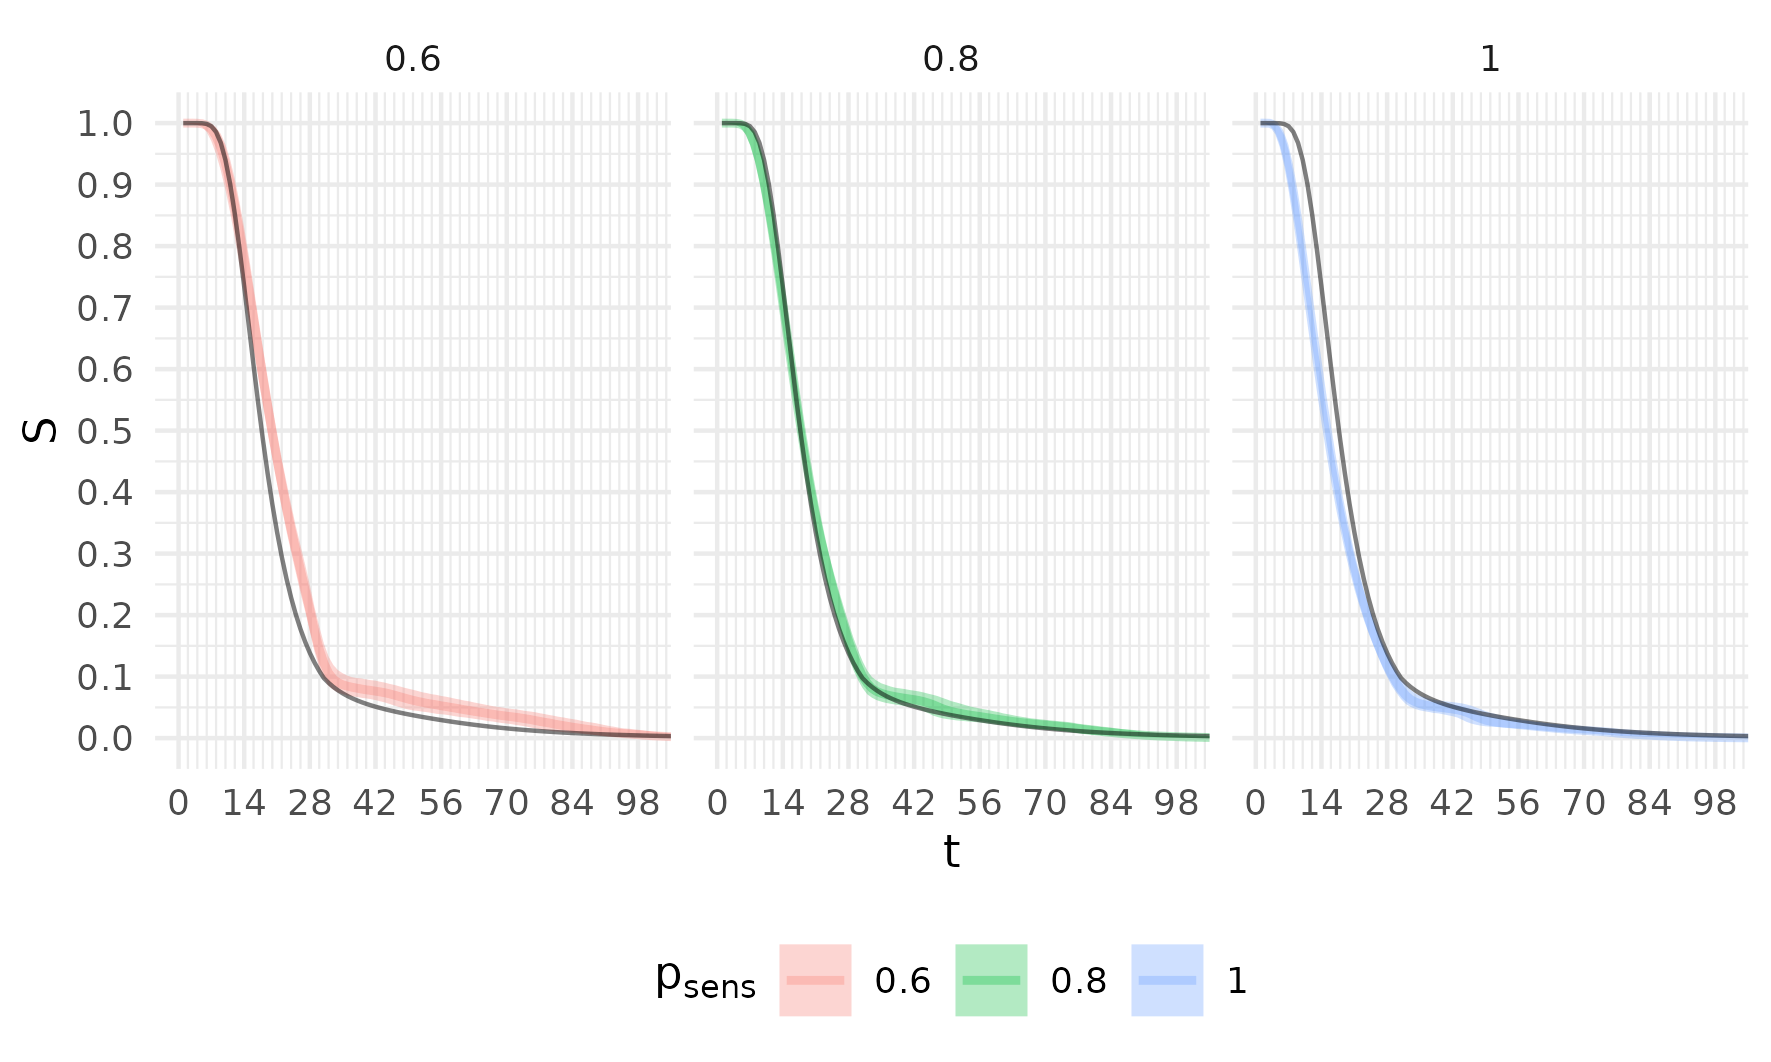
\includegraphics[width=\textwidth]{cis-imperfect-testing/sim-misspecified-sensitivity}
  \caption[Simulation study results with misspecified test sensitivity]{%
    Posterior (median and 95\% credible interval) of the survival time for the simulation study with a possibly misspecified test sensitivity.
    The true survival time is shown in black.
    All results use $\psenss = 0.8$, but $\psensi$ varies, as per panel labels.
    Hence, (B) is correctly specified but (A) and (C) have misspecified $\psens$.
  }
  \label{imperf-test:fig:misspecified-test-sensitivity}
\end{figure}

The results when $\psenss = v$ are similar to $\psenss = 0.8$ (see \cref{imperf-test:fig:variable-test-sensitivity}).
This suggests that the simplified model, with constant test sensitivity, is sufficient for recovering the true survival time.
% Estimating the test sensitivity is not possible without a more complex model, as discussed in \cref{imperf-test:sec:discussion}.
Therefore, I apply the constant test sensitivity model to the real CIS data in the next section.
\begin{figure}
  % \makebox[\textwidth][c]{
    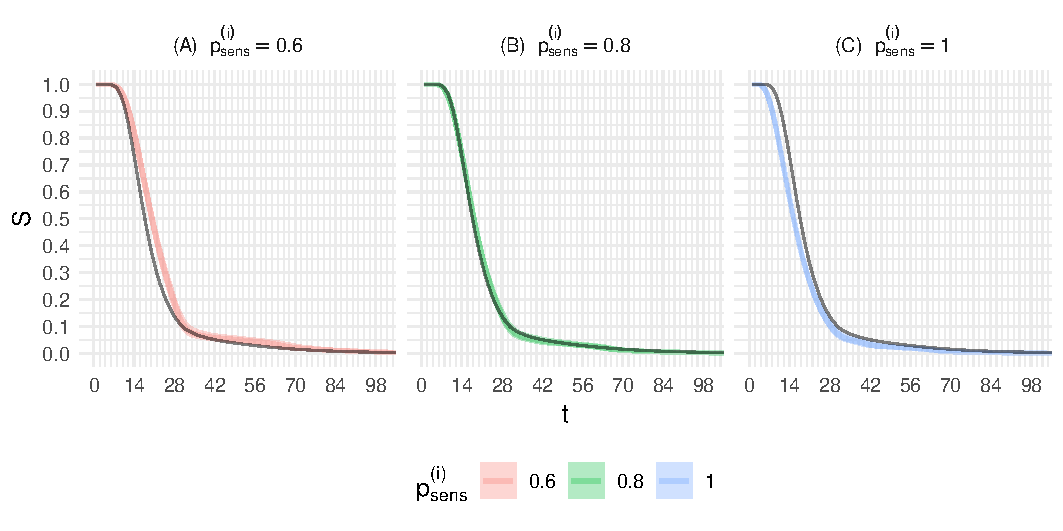
\includegraphics[width=\textwidth]{cis-imperfect-testing/sim-variable-sensitivity}
  \caption[Simulation study results with varying test sensitivity]{%
    Posterior (median and 95\% credible interval) of the survival time for the simulation study with a variable test sensitivity.
    Each panel shows the results of performing inference with a different assumed value for the test sensitivity.
    All results use $\psenss = v$, but $\psensi$ varies, as per panel labels.
  }
  \label{imperf-test:fig:variable-test-sensitivity}
\end{figure}

\section{Application to CIS data} \label{imperf-test:sec:application}

In this section, I apply the approach described in this chapter to the CIS episodes dataset I described in \cref{perf-test:sec:data}.
This is the \numprint{4800} CIS infection episodes first detected between 10 Oct 2020 and 6 Dec 2020 inclusive and have negatives bounding the start and end time of the episode.

Unlike in the simulation studies, an uninformative prior on $\ntot$ led to implausible estimates of the duration distribution.
The uninformative prior led to high posterior estimates of $\ntot$, and hence an implausibly large number of episodes with durations of less than five days.
Therefore, I formed an informative prior for $\ntot$, $\ntot \sim \NBc(\mu\inform, r\inform)$, using pre-existing estimates of the total number of infections to give $\mu\inform$ and $r\inform$.
\Textcite{birrellRTM2} estimated the total number of infections in England over the time period I consider, with posterior mean \numprint{4136368} and standard deviation \numprint{27932}.
% This model gives a posterior mean of \numprint{4136368} cumulative infections in England in the time period I consider, with a posterior standard deviation of \numprint{27932}~\citePersonalComms{Paul Birrell}.
\todo{Insert correct citation for RTM paper 2 once available}
Scaling to the size of the CIS and approximating as a negative binomial gives $\mu\inform = \numprint{25132}$ and $r\inform = \numprint{22047}$.

With this prior, the model produces plausible estimates of the duration distribution (see \cref{imperf-test:fig:cis-estimates}).
This estimate (blue) has more long episodes than the estimate in \cref{E-ATACCC} (red).

The qualitative increase in long episodes is robust to the choice of prior for $\ntot$, the assumed value for $\psens$ (see \cref{imperf-test:fig:cis-sensitivity}), and the choice of prior for the hazards, $\lambda_t$ (see \cref{E-perf-test:sec:parameters-priors}).
However, the survival proportion over the first 4 weeks is sensitive to these choices.
The estimate using a test sensitivity of 0.8 and $\NBc(\mu\inform, r\inform)$ give a median survival time most similar to that of \cref{E-ATACCC}.
\begin{figure}
  \makebox[\textwidth][c]{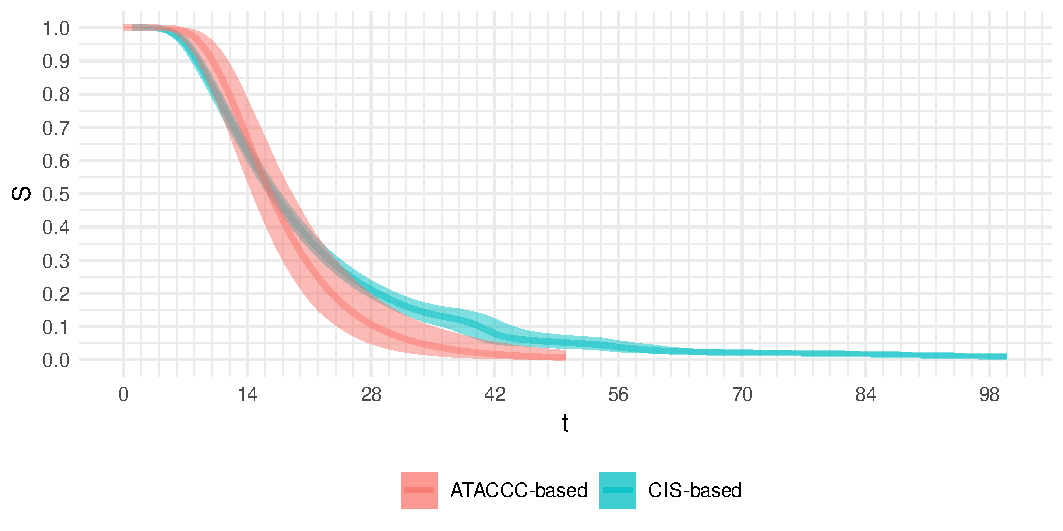
\includegraphics{cis-imperfect-testing/CIS_final}}
  \caption[Comparing estimates of the duration distribution.]{
    Duration estimates using the model in this chapter (CIS) alongside those from \cref{E-ATACCC} (ATACCC).
    Uses the informative prior on $\ntot$, the model combination prior for the hazards, and $\psensi = 0.8$.
  }
  \label{imperf-test:fig:cis-estimates}
\end{figure}
\begin{figure}
  \thisfloatpagestyle{empty}
  \makebox[\textwidth][c]{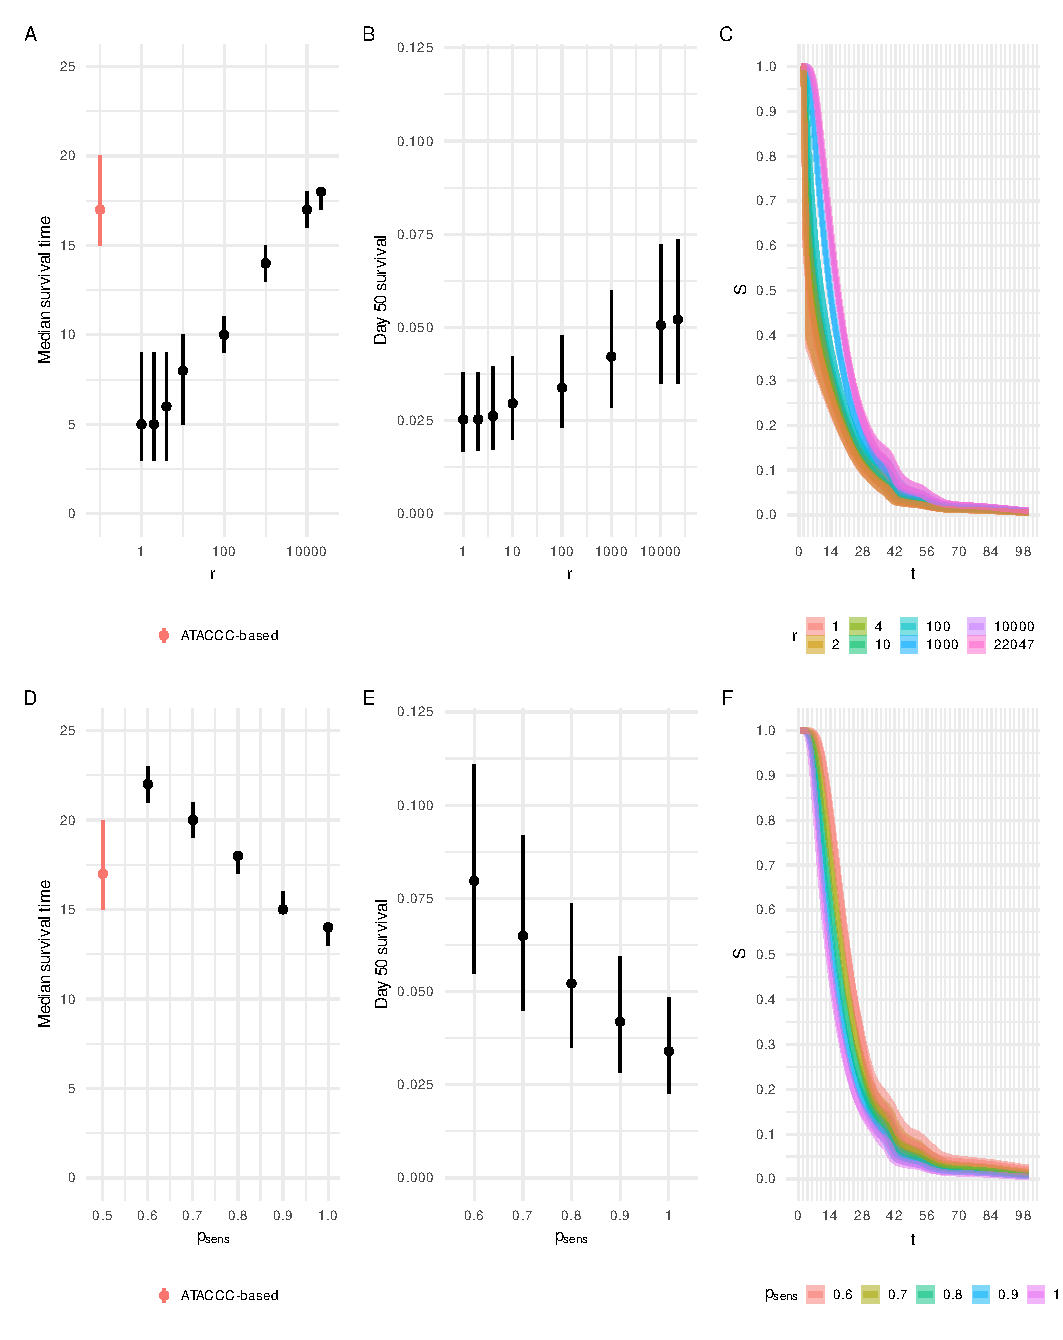
\includegraphics{cis-imperfect-testing/CIS_vary}}
  \caption[Sensitivity of CIS estimates to the prior.]{%
    (A-C) Sensitivity of CIS estimates to the value of $r$, the dispersion of the prior for $\ntot$ (a larger $r$ means a more informative prior) when $\psens = 0.8$.
    (D-F) Sensitivity of CIS estimates to the value of $\psens$ when $r = r\inform$.
    A and D: median survival time, in comparison to the ATACCC-based estimate of \cref{E-ATACCC} (shown in red).
    B and E: survival at day 50, $S_{\vec{\theta}}(50)$.
    C and F: full survival curves out to day 100.
  }
  \label{imperf-test:fig:cis-sensitivity}
  \todo[inline]{Optional improvement: Could highlight the "preferred" model which exists in both rows and is the one used subsequently, and/or include ATACCC in the far-right hand column}
\end{figure}

The estimates are sensitive to the choice of $r$, the strength of the prior on $\ntot$.
A low value for $r$, giving a very weak, almost uninformative, prior on $\ntot$ causes its posterior estimate to be much higher than the estimate from \textcite{birrellRTM2}.
When increasing the prior's strength, the posterior estimate moves towards the prior smoothly, as expected (see \cref{imperf-test:fig:ntot}).
As discussed previously, the \cref{E-ATACCC} estimates are reliable for the first 2--3 weeks, notably including the median time.
The median using $r\inform$ matched \cref{E-ATACCC}'s median estimate and is a principled choice because it is based directly on the prior work \textcite{birrellRTM2}.
Therefore, I use this estimate in the application to the CIS data.
\begin{figure}
  \makebox[\textwidth][c]{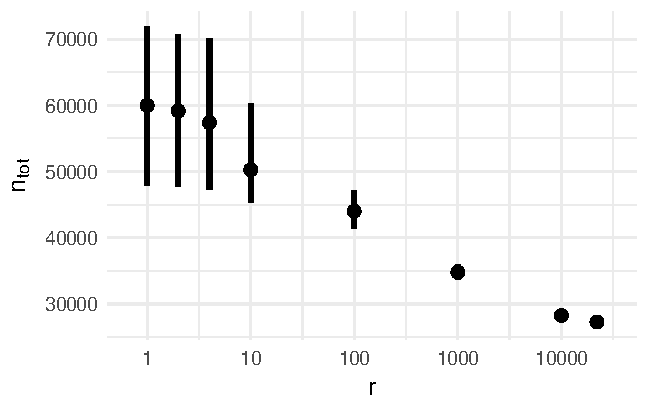
\includegraphics{cis-imperfect-testing/CIS_ntot}}
  \caption[Sensitivity of $\ntot$'s posterior to its prior.]{How the posterior estimate of $\ntot$ changes with the value of $r$ in the prior on $\ntot$.}
  \label{imperf-test:fig:ntot}
\end{figure}

The mean survival time in this final estimate is 21.2 days (95\% CrI: 20.5--21.9), compared to \cref{E-ATACCC}'s estimate of 18.8 days (95\% CrI: 16.5--21.6).
This is a 13\% increase (95\% CrI: 2\% decrease to 29\% increase).

\section{Discussion} \label{imperf-test:sec:discussion}

In this chapter, I developed a novel method to incorporate false negatives into the survival analysis of \cref{E-perf-test}.
I then applied this method to the CIS data, estimating the tail of the duration distribution without the strong model assumptions and extrapolation in \cref{E-ATACCC}.
The qualitative features of the estimated distribution are robust to the assumed value for $\psens$, and the choice of prior for $\lambda$, although the quantitative details are not.
The estimates of the tail, the primary purpose of this chapter, are in addition somewhat robust to the choice of prior for $\ntot$.
The increased estimates in the tail lead to an increased estimate of the mean survival time.
This will decrease estimates of incidence.

Regardless of the assumptions used, a substantial portion of infection episodes last a long time (\eg more than 50 days) (see \cref{imperf-test:fig:cis-estimates,imperf-test:fig:cis-sensitivity}).
This has implications for surveillance because episodes detected by prevalence surveys could have occurred a long time ago.
If an intervention such as a lockdown is implemented, these long episodes could contribute a significant portion to ongoing prevalence levels.
Furthermore, care should be taken when designing testing policies (\eg to release individuals from quarantine or discharge them from hospital) because individuals could test RT-PCR positive for a long time, but cannot be assumed to be infectious.

An informative prior on $\ntot$ is required for the bulk of the distribution to agree with those in \cref{E-ATACCC} and the wider literature.
In the simulation study, the uninformative prior on $\ntot$ performed well, even when the test sensitivity was misspecified.
A possible explanation is that the true variation in the test sensitivity over an episode is significantly different to the function in \cref{imperf-test:eq:variable-test-sensitivity}.
In particular, the test sensitivity for long episodes could be lower than 50\%.
This allows many more episodes to be undetected than the model assumes, and hence a higher $\ntot$ is required to explain the data.
Furthermore, it violates assumptions made in \cref{imperf-test:sec:modelling}; this is similar to the situation in simulation when $\psensi < \psenss$.
Violating these assumptions would lead to unpredictable inference results, perhaps those seen here.

Ideally, the test sensitivity would be estimated from the data.
However, this would require incorporating time-varying test sensitivity into the likelihood.
If the current model, with a constant $\psens$, is used then the estimate of $\psens$ would be heavily informed by intermittent negatives (the first, constant term in \cref{imperf-test:eq:pia-prime}).
These negatives will, in general, be close to the beginning of the episode with a higher test sensitivity than average.

Estimating the test sensitivity excluding intermittent negatives is not possible because \cref{imperf-test:eq:pia-prime-constant,imperf-test:eq:pit-prime} are both monotonically decreasing in $\psens$; therefore, the likelihood always favours $\psens = 0$ (\ie no true positives).
This aligns with the situation with singly interval censored, untruncated data, when stopping at the first observed time of the terminating event (which may be misclassified) means that the test sensitivity cannot be estimated~\autocite[e.g.][]{titmanMisclassify}.

Estimating a time-varying $\psens$ with $S_{\vec{\theta}}$ jointly may cause identifiability issues.
Previous studies have avoided issues by including external information (such as a prior giving the magnitude) on $\psens$, or test results from later follow-up~\autocite[and references therein]{piresIntervalMisclassify}.
However, these studies use a constant $\psens$.
Whether these methods are sufficient for the model to be identifiable with a time-varying $\psens$ needs further investigation.
A simple parametric form of the test sensitivity, such as that proposed by \textcite{brownBayesian}, may be sufficient to allow identifiability.
In any case, the likelihood, especially $p_{iu}'$, would be substantially complicated by such an addition which may greatly increase the computational cost of inference.

The assumption, made in \cref{E-perf-test}, was that the episode start times are independent.
However, because infections are the result of a counting process with intensity shared between individuals (see \cref{E-inc-prev:sec:infection-process}), this assumption is violated.
Prevalence was fairly constant over the period I chose, suggesting the same is true of the incidence.
Additionally, some simulations exploring the results of changing incidence suggested this would not have a large effect on the results (not shown).

% However, comparing the CIS and simulated datasets do not show any differences which suggest what in the data are causing these differences.
% Then, the additional undetected infections implied by a 
% This would lead to more undetected infections than the model assumes, and hence a higher $\ntot$ is required to explain the data.

\section{Conclusion} \label{imperf-test:sec:conclusion}

In this chapter, I developed and applied novel methodology to estimate the duration distribution of RT-PCR positivity using information from two studies: ATACCC and CIS.
The preferred estimates assume a test sensitivity of 0.8 and use an informative prior on the number of infections.

These estimates are the first estimates of the duration of RT-PCR positivity, including the distribution tails, estimated from general population data.
This feature of the distribution is important for understanding the proportion of prevalence attributable to long infections and interpreting RT-PCR test results.

Producing these estimates required applying previous survival analysis frameworks in the novel context of the CIS.
The framework needed further modification to account for the presence of false negatives, done in this chapter.

The posterior distribution for the survival has narrow credible intervals, likely due to the large sample size in the CIS.
In the following chapter, I will take the posterior mean for the survival time at each point, neglecting this uncertainty, as the basis for estimating transmission.
% First, I will take a backcalculation approach (\cref{E-backcalc}), based on the framework in \cref{E-inc-prev}.
% Then, I will take a mechanistic approach (\cref{E-SEIR}), modelling the transmission process explicitly.

\ifSubfilesClassLoaded{
  \listoftodos
}{}

\end{document}